The homogeneous rigid transform is an extremely useful tool used to represent various things in robotics. 
First, the rigid transform is defined as a transformation $T$ that when acting on any vector $v$, produces a transformed vector $T(v)$ of the form: 
\begin{equation}
	T(v) = R v + t
\end{equation}

where $R^T R^{-1}$, and $t$ is a vector giving the translation of the origin. 
This concept can be represented in a form called a {\it homogeneous transformation matrix}. 
A homogeneous transformation matrix $T \in \mathbb{R}^{4 \times 4}$ is a member of special euclidean group $SE(3)$, and can be written in the form:
\begin{equation}
	T = \begin{bmatrix}
		R & t \\
		\bf{0} & 1
	\end{bmatrix}
\end{equation}
where $R \in \mathbb{R}^{3 \times 3}$ is a rotation matrix, and $t \in \mathbb{R}^3$ is a translation vector. 
The inverse of a homogeneous transformation matrix is:
\begin{align}
	T^{-1} &= 
	\begin{bmatrix}
		R^T & -R^Tt \\
		\bf{0} & 1
	\end{bmatrix} \\
	T T^{-1} &= \bf{I}
\end{align}
When using super and subscripts to specify the frames we are referring to, then $T_b^a = (T_a^b)^{-1}$.
We can use a homogeneous transformation to operate on homogeneous points $p, q \in \mathbb{R}^4$, 
\begin{align}
	q &= Tp \\
	\begin{bmatrix} 
		x_q \\ 
		y_q \\
		z_q \\
		1
	\end{bmatrix}
	&= \begin{bmatrix}
		R & t \\
		\bf{0} & 1
	\end{bmatrix} 
	\begin{bmatrix}
		x_p \\
		y_p \\
		z_p \\
		1
	\end{bmatrix}.
\end{align}

In general, there are three interpretations for homogeneous transformations:
\begin{enumerate}
	\item A description of relative orientation and translation between frames. 
	\item A coordinate transform between frames. 
	Specifically, $T_j^i$ is a transform from frame ${j}$ to frame ${i}$:
	\begin{equation}
		P^i = T_j^i P^j
	\end{equation}
	\item A motion of a point (or a collection of points) within a single frame. For example, as we saw above point $p$ can be moved to point $q$:
	\begin{align}
		q &= Tp \\
		P_2^i &= T_j^i P^i_1
	\end{align}
	Similarly, a homogeneous transform can represent a motion from one frame to another.
	Specifically, $T_j^i$ moves frame $i$ to frame $j$. 
\end{enumerate}
It is important to specify which of these interpretations you are using within your program, as it can get confusing what these transformations represent if people aren't on the same page. 

Additionally, one must pay attention to the frame that the operand is in, as this determines the function of the transform to some degree. 
$P_2^i = T^i_j P_1^i$ is a motion that operates on point $P_1^i$ within frame $i$ whereas $P^i = T_j^i P^j$ is a coordinate transformation from $j$ to $i$, and therefore if we feed a point in frame $j$ to this transformation, the point will not move, but the coordinates will be transformed into frame $i$, which is often desired.  

\subsection{Transforming between frames}
We can chain together homogeneous transforms to represent a traversal through frames. 
\begin{figure}[H]
	\centering
	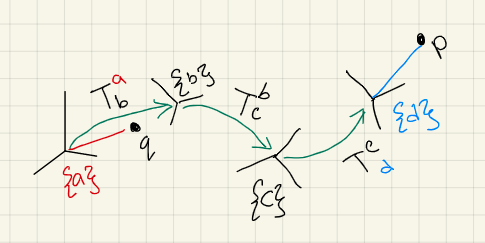
\includegraphics[width=0.8\textwidth]{images/frame_traversal.png}
	\caption{Traversing through different coordinate frames represented by rigid transformation matrices.}
	\label{fig: frames}
\end{figure}

Say we want the transform from $a$ to $d$:
\begin{equation}
	T_d^a = T^a_b T^b_c T^c_d.
\end{equation}
Notice that the bottom subscript and the following top subscript "cancel" out when multiplying frames together. 
Additionally when composing transforms like this, the "source" frame (in this case $d$) is included in the right most transform, and the "destination" frame $a$, is included in the left most. 

Using this knowledge we can represent frames that are related in this way by a pose graph, or pose tree consisting of parent and child relationships between each frame. 

\begin{figure}[H]
	\centering
	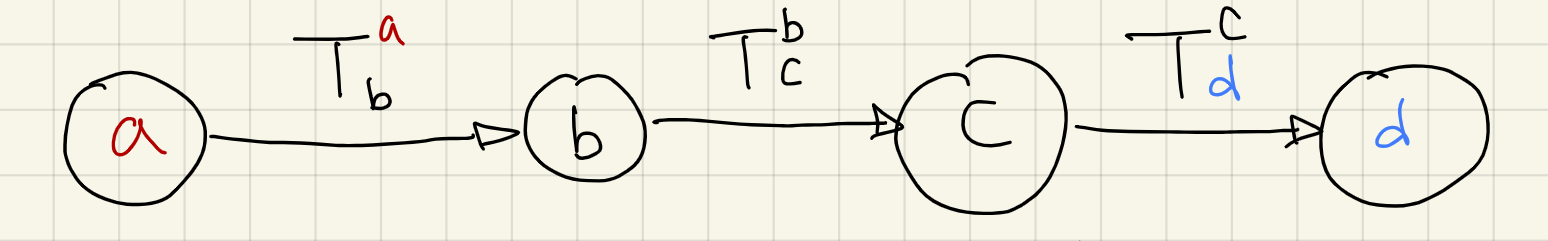
\includegraphics[width=0.8\textwidth]{images/pose_graph.png}
	\caption{Frames and their transforms can be represented in graph form.}
	\label{fig: poses}
\end{figure}